% The Slide Definitions
%document
\documentclass[10pt]{beamer}
%theme
\usetheme{metropolis}
% packages
\usepackage{color}
\usepackage{listings}
\usepackage[ngerman]{babel}
\usepackage[utf8]{inputenc}
\usepackage{multicol}

\usepackage{hyperref}
\hypersetup{colorlinks=true, linkcolor=blue, urlcolor=red}

% color definitions
\definecolor{mygreen}{rgb}{0,0.6,0}
\definecolor{mygray}{rgb}{0.5,0.5,0.5}
\definecolor{mymauve}{rgb}{0.58,0,0.82}

\lstset{
    backgroundcolor=\color{white},
    % choose the background color;
    % you must add \usepackage{color} or \usepackage{xcolor}
    basicstyle=\footnotesize\ttfamily,
    % the size of the fonts that are used for the code
    breakatwhitespace=false,
    % sets if automatic breaks should only happen at whitespace
    breaklines=true,                 % sets automatic line breaking
    captionpos=b,                    % sets the caption-position to bottom
    commentstyle=\color{mygreen},    % comment style
    % deletekeywords={...},
    % if you want to delete keywords from the given language
    extendedchars=true,
    % lets you use non-ASCII characters;
    % for 8-bits encodings only, does not work with UTF-8
    frame=single,                    % adds a frame around the code
    keepspaces=true,
    % keeps spaces in text,
    % useful for keeping indentation of code
    % (possibly needs columns=flexible)
    keywordstyle=\color{blue},       % keyword style
    % morekeywords={*,...},
    % if you want to add more keywords to the set
    numbers=left,
    % where to put the line-numbers; possible values are (none, left, right)
    numbersep=5pt,
    % how far the line-numbers are from the code
    numberstyle=\tiny\color{mygray},
    % the style that is used for the line-numbers
    rulecolor=\color{black},
    % if not set, the frame-color may be changed on line-breaks
    % within not-black text (e.g. comments (green here))
    stepnumber=1,
    % the step between two line-numbers.
    % If it's 1, each line will be numbered
    stringstyle=\color{mymauve},     % string literal style
    tabsize=4,                       % sets default tabsize to 4 spaces
    % show the filename of files included with \lstinputlisting;
    % also try caption instead of title
    language = C,
	showspaces = false,
	showtabs = false,
	showstringspaces = false,
	escapechar = ,
}

\def\ContinueLineNumber{\lstset{firstnumber=last}}
\def\StartLineAt#1{\lstset{firstnumber=#1}}
\let\numberLineAt\StartLineAt



\newcommand{\codeline}[1]{
	\alert{\texttt{#1}}
}


% Author and Course information
% This Document contains the information about this course.

% Authors of the slides
\author{
    Lecturers:
	%name1
	Mirko Jantschke,
	%name2
	Pascal Scholz
	\\
	%creaters of the slides
	Created by: Richard Mörbitz, Manuel Thieme
}


% Fancy Logo
\titlegraphic{\hfill
\includegraphics[height=1.25cm]{../templates/fsr_logo_cropped}}


% Presentation title
% TODO Change the topic of the lesson
\title{Ersatzkurs 2}
\date{\today}


\begin{document}

\maketitle

\begin{frame}{Gliederung}
	\setbeamertemplate{section in toc}[sections numbered]
	\tableofcontents
\end{frame}

%-----------------------------------------------------------------------------------------------
\section{Closer look at main}
%-----------------------------------------------------------------------------------------------

\begin{frame}[fragile]{Main with arguments}
    The main function does have arguments
    \begin{itemize}
     \item \textit{argc} which is the the count of the given arguments.
     \item \textit{argv} which is basically an array with the arguments.
    \end{itemize}

    \begin{lstlisting}[numbers=left]
int main(int argc, char** agrv) {
	/*Code*/
	return expression;
}    \end{lstlisting}

    The first entry in \textit{argv} is the path of the program. 
\end{frame}

%-----------------------------------------------------------------------------------------------

\begin{frame}[fragile]{Example}
    Running a program \textit{a.c}:
    \begin{lstlisting}[numbers=left]
int main(int argc, char** agrv) {
	int a = 0;
	while(a < argc){
        printf("Argument number %d is: %s\n", a, argv[a]);
        ++a; 
	}
}    \end{lstlisting}
    will result in the output:    
    \begin{lstlisting}[numbers=left]
    $ ./a.out firstArg secondArg
        Argument number 0 is ./a
        Argument number 1 is firstArg
        Argument number 2 is secondArg  \end{lstlisting}
\end{frame}

%-----------------------------------------------------------------------------------------------

\begin{frame}{Task 1}
    Write a programm with the shown main function which takes two file names as arguments and 
    and print both.  
\end{frame}

%-----------------------------------------------------------------------------------------------
\section{File I/O}
%-----------------------------------------------------------------------------------------------

\begin{frame}[fragile]{stdio.h with more functions}
    You already used the header \textit{stdio.h}.
    It contains much more than \textit{pritnf()} and \textit{scanf()}.
    With the command
    \begin{lstlisting}[numbers=left]
    $ man stdio.h \end{lstlisting}    
    you can view the linux man(ual) pages which is the documentation for this files.
    \newline
    You can use any type of online documentation too.
\end{frame}

%-----------------------------------------------------------------------------------------------

\begin{frame}[fragile]{stdio.h with more functions}
    \centerline{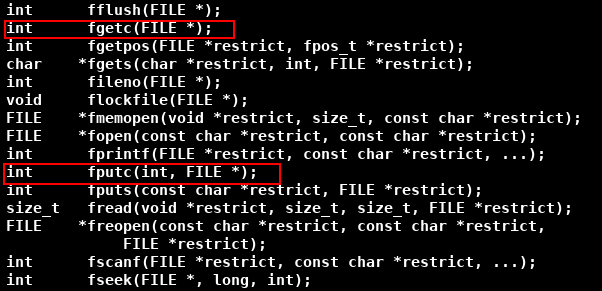
\includegraphics[scale=.7]{../img/man.png}}
    We will use the functions \textit{fegtc} and \textit{fputc}.
\end{frame}

%-----------------------------------------------------------------------------------------------

\begin{frame}[fragile]{How do they work}
    Both functions take a pointer of type FILE* which they will work with. 
    \newline
    \newline
    \textit{fgetc()} will return the ASCII number of the read char.
    \newline
    \newline
    \textit{fputc()} takes additionally the number which will be written. 
    \newline
    \newline
    Both will return an error code if something wents wrong. So check the returned value!
    \newline
    \newline
    To open a file use \textit{fopen()} and to close a file after you are done use \textit{fclose()}.
\end{frame}

%-----------------------------------------------------------------------------------------------

\begin{frame}[fragile]{Example}
    The following example will open a file, read and print a byte:
    \begin{lstlisting}[numbers=left]
int main(int argc, char** agrv) {
	FILE *fp;
	int buff;
	char * fname;
	if(argc > 1)
        fname = argv[1];
	//open file
	if( access( fname, F_OK ) != -1 ) {
        fp = fopen(fname, "r");
        if((buff = fgetc((FILE*) fp)) != EOF)
            printf("The char which was read: %c", buff);        
	}else{
        printf("Could not open file\n");
        return -1;
	}
	return 0;
}   \end{lstlisting}
\end{frame}

\begin{frame}{Task}
    You already got a programm which can handle arguments.\newline
    \newline
    Write a file test.csv with the contents: 4,5,6
    \newline
    Now your programm should except to be called with a file name. Open this file, read and then print the first line. The ASCII-Code for the line ending used in POSIX Systems is 10.
\end{frame}

\begin{frame}{File format}
    We define our file format to have the dimensions given in the first line.
    The lines after th first line are values.\newline
\end{frame}


\end{document}
